\section{Budget estimation}

For this section I am going to present an estimation of the budget needed to make 
the project possible. The costs will be divided in three groups depending on their 
type. These types are software, hardware and human resources.

To calculate the amortization I'll consider the useful life of the resource and that 
the project will last 56 days, following the planning.

\subsection{Hardware resources}

The table below lists the hardware resources needed for the realization of the project, 
their cost and amortization.
\begin{figure}[H]
    \centering
    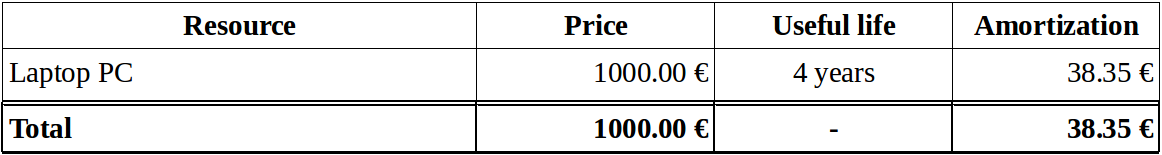
\includegraphics[width=\textwidth]{hardware_res}
    \caption{Hardware resources}
    \label{fig:hardware_res}
\end{figure}

\subsection{Software resources}

The next table lists the software resources needed for the project in the same format 
as the previous section.
\begin{figure}[H]
    \centering
    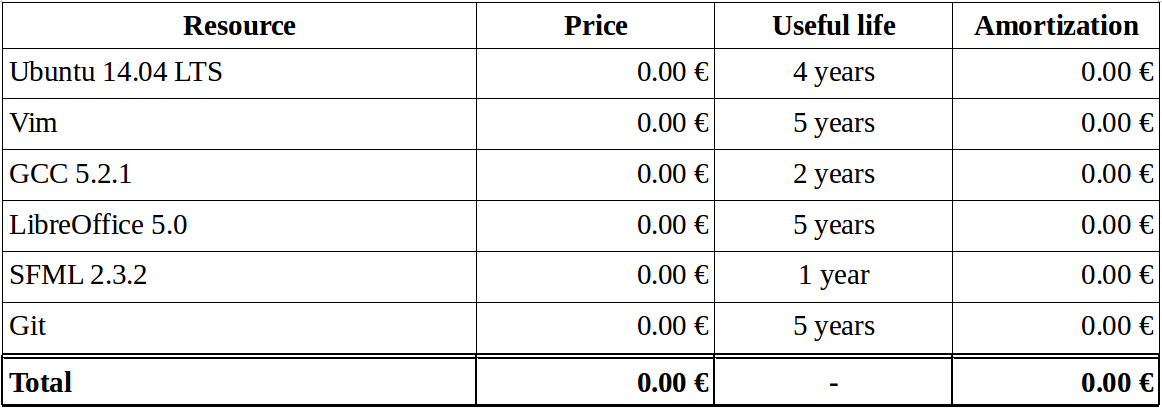
\includegraphics[width=\textwidth]{software_res}
    \caption{Software resources}
    \label{fig:software_res}
\end{figure}

\subsection{Human resources}

The table shows the costs for the human resources needed in the development of the 
project. The cost is calculated assuming a 4 hours per day schedule.
\begin{figure}[H]
    \centering
    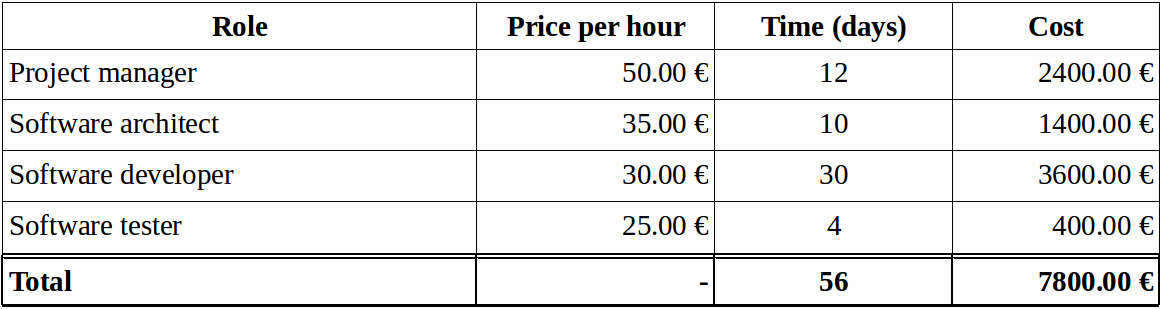
\includegraphics[width=\textwidth]{human_res}
    \caption{Human resources}
    \label{fig:human_res}
\end{figure}

Each of these different roles will be assigned different tasks in the project. Specifically, 
the \textit{Project manager} will be assigned to almost the whole \textit{Project 
planning} task and the \textit{Final task}; the \textit{Software architect} will work 
at the ending part of the \textit{Project planning} determining the blueprints for 
the development of the project; the \textit{Software developer} will take care of 
the whole development; and the \textit{Software tester} will test the project when 
new milestones are reached during the development task.

\subsection{Total budget}

From the estimations in previous sections the following summary can be obtained, showing 
the total budget for the development of the project.

\begin{figure}[h]
    \centering
    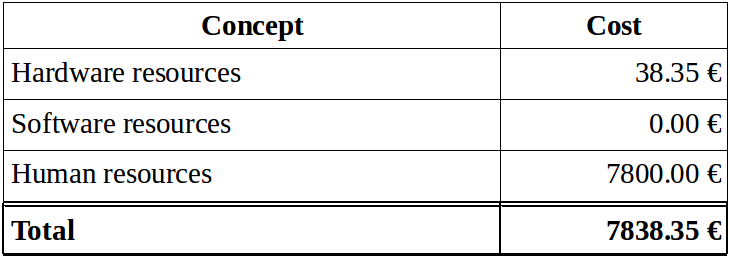
\includegraphics[width=0.7\textwidth]{total_budget}
    \caption{Total budget}
    \label{fig:total_budget}
\end{figure}

\subsection{Budget control}

The budget estimation as its name says is an estimation, therefore is not rigid and 
prone to changes.

The tasks that are more susceptible to deviations from the planning are the ones related 
to software architecture and development. If at any point there is a substantial delay 
in the development, the software developer will need to be hired for extra hours, 
thus changing the budget. On the other hand, I am confident with the planning and 
I don't expect any big deviation from it.
